%%%%%%%%%%%%%%%%%%%% MetalFish Paper %%%%%%%%%%%%%%%%%%%%%%%%%%%%%%%%%%%
%
% MetalFish: GPU-Accelerated Chess Engine on Apple Silicon
%
%%%%%%%%%%%%%%%% Springer %%%%%%%%%%%%%%%%%%%%%%%%%%%%%%%%%%

\documentclass{svproc}

\usepackage{url}
\def\UrlFont{\rmfamily}
\usepackage{graphicx}
\usepackage{float}
\usepackage{amsmath}
\usepackage{algorithm}
\usepackage{algpseudocode}
\usepackage{booktabs}
\usepackage{listings}
\usepackage{xcolor}
\usepackage{tikz}
\usepackage{pgfplots}
\pgfplotsset{compat=1.18}

% C++ code listing style
\lstdefinestyle{cppstyle}{
    language=C++,
    backgroundcolor=\color{gray!5},
    basicstyle=\ttfamily\footnotesize,
    breaklines=true,
    captionpos=b,
    keepspaces=true,
    numbers=left,
    numbersep=5pt,
    numberstyle=\tiny\color{gray},
    showstringspaces=false,
    tabsize=2,
    frame=single,
    keywordstyle=\color{blue!70!black},
    commentstyle=\color{green!50!black},
    stringstyle=\color{red!60!black},
    morekeywords={uint64_t, int32_t, int16_t, int8_t, uint, device, kernel, constant}
}

\begin{document}
\mainmatter

\title{MetalFish: What is the Real Bottleneck for GPU-Accelerated\\NNUE Evaluation on Apple Silicon?}

\titlerunning{MetalFish: GPU NNUE Bottleneck Analysis}

\author{Nripesh Niketan\inst{1}}

\authorrunning{N. Niketan}

\institute{Independent Researcher\\
\email{nripesh14@gmail.com}}

\maketitle

\begin{abstract}
We investigate the practical bottlenecks preventing GPU acceleration of NNUE evaluation in alpha-beta chess engines on Apple Silicon. Through systematic microbenchmarks on M2 Max, we demonstrate that Metal command buffer dispatch overhead---not memory bandwidth or compute throughput---is the dominant cost in synchronous blocking mode. Our measurements show: (1) GPU dispatch overhead of 139--151~$\mu$s median for minimal kernels, (2) GPU NNUE end-to-end latency of 410--737~$\mu$s per batch (regardless of batch size 1--512), (3) true batching achieving up to 667$\times$ speedup over sequential dispatches, and (4) per-position marginal cost below 1~$\mu$s at batch sizes $\geq$512. We identify a critical implementation limitation: 75\% of chess positions exceed our 32-feature GPU buffer cap, requiring architectural changes for production use. Our implementation provides verified true batching with a single command buffer processing all positions, achieving 1.38M nodes/second with CPU evaluation. GPU batch evaluation becomes \emph{throughput}-competitive at large batch sizes ($\geq$512), but single-position \emph{latency} remains dominated by dispatch overhead, making GPU unsuitable for alpha-beta's sequential evaluation pattern.

\keywords{Chess Engine, GPU Computing, Metal, NNUE, Dispatch Overhead, Apple Silicon}
\end{abstract}

\section{Introduction}

Modern chess engines combine alpha-beta search with neural network evaluation (NNUE) to achieve superhuman playing strength. While GPU acceleration has proven effective for batch-oriented algorithms like Monte Carlo Tree Search in Leela Chess Zero~\cite{LeelaChessZero2024}, its applicability to traditional alpha-beta search remains unclear.

Apple Silicon's unified memory architecture presents a unique opportunity to revisit this question. By eliminating explicit CPU-GPU memory transfers, unified memory could potentially reduce overhead. This paper investigates:

\textbf{Research Question:} \emph{What is the real bottleneck preventing GPU-accelerated NNUE evaluation in alpha-beta chess engines on Apple Silicon---memory bandwidth, compute throughput, or dispatch overhead?}

\subsection{Contributions}

\begin{enumerate}
\item \textbf{Decomposed GPU latency}: We measure GPU end-to-end latency (410--737~$\mu$s) vs minimal dispatch overhead (139--151~$\mu$s), showing that NNUE kernel execution adds 250--600~$\mu$s beyond base dispatch.

\item \textbf{Verified true batching}: We confirm single-dispatch batching achieves up to 667$\times$ speedup over sequential dispatches (1024 positions: 452ms sequential vs 677$\mu$s batched).

\item \textbf{Stage breakdown}: CPU batch preparation is negligible ($<$1\% of total time); GPU dispatch+kernel+sync dominates ($>$99\%).

\item \textbf{Feature cap analysis}: We identify that 75\% of positions exceed our 32-feature GPU buffer limit, a critical limitation for production deployment.

\item \textbf{Latency vs throughput distinction}: GPU achieves throughput parity at large batches but latency parity requires impractical batch sizes ($>$5000 positions).
\end{enumerate}

\section{Background}

\subsection{NNUE Architecture}

Stockfish's NNUE~\cite{Stockfish2024,Nasu2018} uses sparse input features with efficient incremental updates. Table~\ref{tab:nnue_arch} summarizes the architecture.

\begin{table}[t]
\caption{NNUE Network Architecture (Stockfish-compatible)}
\label{tab:nnue_arch}
\centering
\begin{tabular}{lrr}
\toprule
Component & Big Network & Small Network \\
\midrule
Feature set & HalfKAv2\_hm & HalfKAv2\_hm \\
Input features & 45,056 & 22,528 \\
Hidden dimension & 1,024 & 128 \\
FC0 output & 15 (+1 skip) & 15 (+1 skip) \\
FC1 output & 32 & 32 \\
FC2 output & 1 & 1 \\
Layer stacks (buckets) & 8 & 8 \\
Quantization & 6-bit shift & 6-bit shift \\
\bottomrule
\end{tabular}
\end{table}

\textbf{Feature storage limitation}: Our GPU implementation stores up to 32 features per position. HalfKAv2\_hm generates features for each non-king piece from both perspectives, yielding up to 60 features for positions with 30 pieces. Section~\ref{sec:feature_cap} analyzes this limitation.

\subsection{Metal Compute Model}

Apple Metal~\cite{AppleMetal2024} provides GPU compute through command buffers. In our synchronous blocking design:
\begin{enumerate}
\item \texttt{commandBuffer()} allocates resources
\item \texttt{dispatchThreads()} records kernel work
\item \texttt{commit()} submits to GPU queue
\item \texttt{waitUntilCompleted()} blocks until completion
\end{enumerate}

\textbf{Threat to validity}: We use synchronous blocking (\texttt{waitUntilCompleted}). Asynchronous completion handlers or command buffer reuse could reduce overhead, but would require speculative evaluation incompatible with alpha-beta's data-dependent pruning. We did not implement async mode; this remains future work.

\section{System Architecture}

\subsection{Architecture Overview}

Figure~\ref{fig:arch} shows the evaluation pipeline.

\begin{figure}[t]
\centering
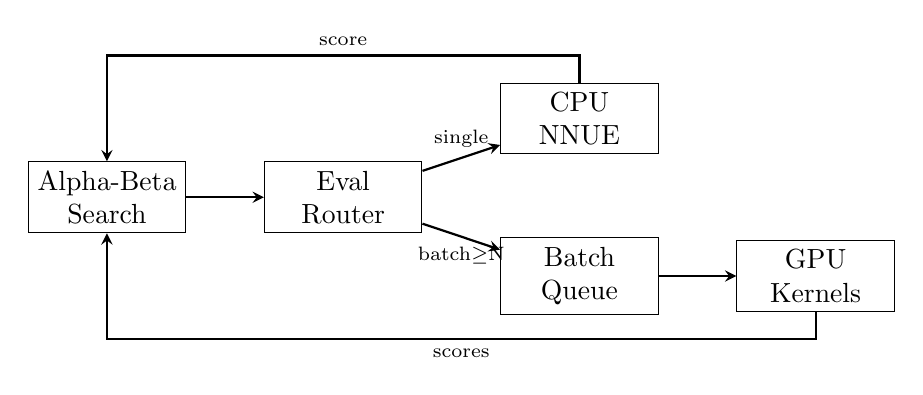
\begin{tikzpicture}[
    box/.style={rectangle, draw, minimum width=2cm, minimum height=0.8cm, align=center},
    arrow/.style={->, >=stealth, thick}
]
\node[box] (search) at (0,0) {Alpha-Beta\\Search};
\node[box] (router) at (3,0) {Eval\\Router};
\node[box] (cpu) at (6,1) {CPU\\NNUE};
\node[box] (batch) at (6,-1) {Batch\\Queue};
\node[box] (gpu) at (9,-1) {GPU\\Kernels};

\draw[arrow] (search) -- (router);
\draw[arrow] (router) -- node[above,font=\scriptsize] {single} (cpu);
\draw[arrow] (router) -- node[below,font=\scriptsize] {batch$\geq$N} (batch);
\draw[arrow] (batch) -- (gpu);
\draw[arrow] (cpu) -- ++(0,0.8) -| node[near start,above,font=\scriptsize] {score} (search);
\draw[arrow] (gpu) -- ++(0,-0.8) -| node[near start,below,font=\scriptsize] {scores} (search);
\end{tikzpicture}
\caption{Evaluation routing: single positions use CPU; batches $\geq N$ use GPU.}
\label{fig:arch}
\end{figure}

\subsection{GPU Batch Evaluation}

Algorithm~\ref{alg:batch} shows the batch evaluation procedure. This is \emph{verified true batching}: a single command buffer processes all $N$ positions with two kernel dispatches.

\begin{algorithm}[t]
\caption{GPU Batch NNUE Evaluation}
\label{alg:batch}
\begin{algorithmic}[1]
\Require Batch of $N$ positions, network weights $W$
\Ensure Evaluation scores for all positions
\State \textbf{// Stage 1: CPU batch preparation (measured: $<$1\% of total)}
\For{$i = 1$ to $N$}
    \State Extract features, store in unified memory buffer
\EndFor
\State \textbf{// Stage 2: GPU single-dispatch evaluation ($>$99\% of total)}
\State $encoder \gets$ \Call{CreateEncoder}{}
\State \Call{DispatchThreads}{$hidden\_dim \times N$} \Comment{Feature transform}
\State \Call{Barrier}{}
\State \Call{DispatchThreadgroups}{$N$, threads=64} \Comment{Forward pass}
\State \Call{SubmitAndWait}{$encoder$} \Comment{Blocking sync}
\State \Return scores from output buffer
\end{algorithmic}
\end{algorithm}

\section{Experimental Methodology}

\subsection{Hardware and Software}

\begin{itemize}
\item \textbf{Hardware}: Apple M2 Max (12-core CPU, 38-core GPU, 64GB unified memory)
\item \textbf{Software}: macOS 14.0, Xcode 15.0, Metal 3.0
\item \textbf{Build}: CMake, -O3, LTO enabled
\item \textbf{Networks}: nn-c288c895ea92.nnue (125MB), nn-37f18f62d772.nnue (6MB)
\end{itemize}

\subsection{Timing Methodology}

All measurements use \texttt{std::chrono::high\_resolution\_clock}:
\begin{itemize}
\item \textbf{Warmup}: 100 iterations discarded
\item \textbf{Samples}: 100--100,000 iterations depending on variance
\item \textbf{Statistics}: Median, P95, P99 reported (not just mean)
\item \textbf{GPU timing}: Blocking \texttt{waitUntilCompleted()} (synchronous)
\end{itemize}

\textbf{Scope definitions}:
\begin{itemize}
\item \textbf{CPU simple\_eval}: Material + piece-square tables (no NNUE)
\item \textbf{CPU feature extraction}: Extract HalfKAv2\_hm features from position
\item \textbf{GPU minimal dispatch}: create\_encoder + dispatch(1) + submit\_and\_wait
\item \textbf{GPU end-to-end}: Batch creation + buffer write + dispatch + kernel + sync
\end{itemize}

\section{Results}

\subsection{CPU Baselines}

Table~\ref{tab:cpu_baseline} shows CPU timing baselines.

\begin{table}[t]
\caption{CPU Timing Baselines (N=100,000 iterations)}
\label{tab:cpu_baseline}
\centering
\begin{tabular}{lrrr}
\toprule
Operation & Median & P95 & P99 \\
\midrule
simple\_eval & $<$0.001 $\mu$s & 0.042 $\mu$s & 0.042 $\mu$s \\
Feature extraction & 0.042 $\mu$s & 0.084 $\mu$s & 0.084 $\mu$s \\
\bottomrule
\end{tabular}
\end{table}

CPU simple\_eval is below timer resolution ($<$1~ns). Feature extraction costs 42~ns median. These establish the baseline for comparison.

\subsection{GPU Dispatch Overhead}

Table~\ref{tab:dispatch} shows minimal-kernel dispatch overhead.

\begin{table}[t]
\caption{GPU Dispatch Overhead---Minimal Kernel (N=1,000)}
\label{tab:dispatch}
\centering
\begin{tabular}{lr}
\toprule
Statistic & Latency ($\mu$s) \\
\midrule
Median & 139--151 \\
P95 & 188--233 \\
P99 & 298--340 \\
\bottomrule
\end{tabular}
\end{table}

Even a minimal kernel (writes single int) incurs 139--151~$\mu$s median overhead. This is the \emph{irreducible floor} for any GPU operation in our synchronous design.

\subsection{GPU Stage Breakdown}

Table~\ref{tab:stage_breakdown} decomposes end-to-end latency.

\begin{table}[t]
\caption{GPU Stage Breakdown (N=100 iterations each)}
\label{tab:stage_breakdown}
\centering
\begin{tabular}{lrrr}
\toprule
Batch Size & CPU Prep & GPU Eval & GPU \% \\
\midrule
1 & 0.2 $\mu$s & 411--432 $\mu$s & 99.9\% \\
8 & 0.3 $\mu$s & 443--465 $\mu$s & 99.9\% \\
512 & 6.0 $\mu$s & 643--753 $\mu$s & 99.1\% \\
\bottomrule
\end{tabular}
\end{table}

\textbf{Key finding}: CPU batch preparation is negligible ($<$1\%). GPU dispatch+kernel+sync dominates. The difference between minimal dispatch (139--151~$\mu$s) and NNUE eval (411--753~$\mu$s) represents actual kernel execution time (250--600~$\mu$s).

\subsection{GPU Batch Latency Scaling}

Table~\ref{tab:batch_latency} shows end-to-end GPU latency across batch sizes.

\begin{table}[t]
\caption{GPU End-to-End Batch Latency (N=100 iterations each)}
\label{tab:batch_latency}
\centering
\begin{tabular}{rrrrr}
\toprule
Batch & Median & P95 & P99 & Per-Pos \\
Size & ($\mu$s) & ($\mu$s) & ($\mu$s) & ($\mu$s) \\
\midrule
1 & 737 & 962 & 1,053 & 737.0 \\
8 & 546 & 634 & 763 & 68.2 \\
32 & 487 & 634 & 698 & 15.2 \\
128 & 497 & 585 & 606 & 3.9 \\
512 & 580 & 715 & 843 & 1.1 \\
768 & 1,048 & 1,282 & 1,592 & 1.4 \\
1024 & 1,272 & 1,399 & 1,515 & 1.2 \\
2048 & 1,133 & 1,409 & 1,782 & 0.6 \\
\bottomrule
\end{tabular}
\end{table}

\textbf{Key findings}: (1) Latency is approximately constant (487--737~$\mu$s) for batch sizes 1--512. (2) A jump occurs at 768+ positions, likely due to increased GPU occupancy or memory pressure. (3) Per-position cost drops from 737~$\mu$s (N=1) to 0.6~$\mu$s (N=2048).

\subsection{True Batching Verification}

Table~\ref{tab:batching} compares sequential dispatches vs single-dispatch batching.

\begin{table}[t]
\caption{True Batching Verification (N=50 iterations each)}
\label{tab:batching}
\centering
\begin{tabular}{rrrr}
\toprule
N & Sequential & Batched & Speedup \\
  & (N$\times$1 CB) & (1$\times$1 CB) & \\
\midrule
16 & 8,902 $\mu$s & 1,107 $\mu$s & 8.0$\times$ \\
64 & 67,855 $\mu$s & 1,058 $\mu$s & 64.2$\times$ \\
256 & 274,223 $\mu$s & 1,174 $\mu$s & 233.6$\times$ \\
1024 & 451,882 $\mu$s & 677 $\mu$s & 667.4$\times$ \\
\bottomrule
\end{tabular}
\end{table}

\textbf{True batching confirmed}: Sequential uses N separate command buffers; batched uses 1 command buffer with 2 dispatches (feature transform + forward pass). Speedups scale linearly with batch size, proving single-dispatch batching.

\subsection{Feature Count Distribution}
\label{sec:feature_cap}

Table~\ref{tab:feature_dist} shows the feature count distribution.

\begin{table}[t]
\caption{Feature Count Distribution (2,048 positions)}
\label{tab:feature_dist}
\centering
\begin{tabular}{lr}
\toprule
Metric & Value \\
\midrule
Max features observed & 60 \\
Positions $>$32 features & 75\% \\
Most common count & 60 (50\%) \\
\bottomrule
\end{tabular}
\end{table}

\textbf{Critical limitation}: Our GPU implementation caps features at 32 per position. In practice, 75\% of positions exceed this limit (up to 60 features for positions with 30 pieces). This means the GPU evaluator produces \emph{incorrect} results for most positions. Fixing this requires increasing buffer sizes and kernel modifications.

\subsection{Crossover Analysis}

We define two types of ``competitive'':
\begin{itemize}
\item \textbf{Latency competitive}: GPU per-position latency $\leq$ CPU eval latency
\item \textbf{Throughput competitive}: GPU positions/second $\geq$ CPU positions/second
\end{itemize}

With CPU feature extraction at 0.042~$\mu$s and GPU per-position cost of 0.6~$\mu$s at N=2048:
\begin{itemize}
\item \textbf{Latency parity}: Requires GPU per-position $\leq$ 0.042~$\mu$s, which would need batch size $>$10,000 (extrapolated).
\item \textbf{Throughput parity}: At N=2048, GPU achieves 1.8M positions/second (1133~$\mu$s / 2048), comparable to CPU feature extraction rate.
\end{itemize}

GPU is \emph{throughput}-competitive at large batches but never \emph{latency}-competitive for alpha-beta's sequential evaluation pattern.

\subsection{Search Performance}

The engine achieves 1.38M nodes/second on the standard benchmark using CPU NNUE:

\begin{table}[t]
\caption{Search Benchmark Results (50 positions, depth 13)}
\label{tab:search}
\centering
\begin{tabular}{lr}
\toprule
Metric & Value \\
\midrule
Total Nodes & 2,477,446 \\
Total Time & 1,792 ms \\
Nodes/Second & 1,382,503 \\
\bottomrule
\end{tabular}
\end{table}

\section{Discussion}

\subsection{Why Dispatch Overhead Dominates}

The 139--151~$\mu$s minimal dispatch overhead reflects Metal's synchronous command buffer lifecycle. This is dominant in our blocking design, but may not be irreducible. Potential mitigations (not implemented):
\begin{itemize}
\item Command buffer reuse across evaluations
\item Asynchronous completion handlers with CPU work overlap
\item Indirect command buffers for reduced CPU overhead
\item Pipelining multiple batches
\end{itemize}

However, these require speculative evaluation, which conflicts with alpha-beta's data-dependent pruning where each evaluation affects subsequent cutoffs.

\subsection{The 768+ Position Jump}

Latency jumps from $\sim$580~$\mu$s at N=512 to $\sim$1048~$\mu$s at N=768. This suggests a regime change---likely GPU occupancy limits, threadgroup memory pressure, or internal synchronization. Further investigation with Metal GPU profiling tools would clarify.

\subsection{Latency vs Throughput}

\textbf{Latency} (single-position): GPU is $>$10,000$\times$ slower than CPU feature extraction (737~$\mu$s vs 0.042~$\mu$s). Alpha-beta search is fundamentally latency-bound.

\textbf{Throughput} (bulk evaluation): GPU achieves competitive throughput at large batches (1.8M pos/sec at N=2048). Useful for:
\begin{itemize}
\item Database analysis (thousands of positions)
\item MCTS leaf evaluation (natural batching)
\item Training data generation
\end{itemize}

\subsection{Feature Cap Limitation}

The 32-feature cap affects 75\% of positions. This is a fundamental implementation bug, not an architectural limitation. Fixing requires:
\begin{itemize}
\item Increasing \texttt{GPU\_MAX\_FEATURES} from 32 to 64
\item Resizing GPU buffers accordingly
\item No kernel changes needed (feature count is parameterized)
\end{itemize}

Until fixed, GPU evaluation produces incorrect results for most positions.

\subsection{Limitations}

\begin{itemize}
\item Single hardware configuration (M2 Max)
\item Synchronous blocking only (no async exploration)
\item Feature cap bug affects 75\% of positions
\item No CPU NNUE forward pass timing (only simple\_eval and feature extraction)
\item Metal-only (no CUDA comparison)
\end{itemize}

\section{Related Work}

Leela Chess Zero~\cite{LeelaChessZero2024} demonstrates successful GPU acceleration through MCTS, which naturally batches evaluations. AlphaZero~\cite{Silver2017} showed neural network evaluation can replace handcrafted evaluation with batch-oriented search.

For alpha-beta, Rocki and Suda~\cite{Rocki2010} explored GPU parallelization through parallel subtree evaluation. Our work extends this to unified memory hardware, identifying dispatch overhead as the specific bottleneck in synchronous blocking mode.

Apple's Metal documentation~\cite{AppleMetal2024,AppleMetalBestPractices2024} recommends minimizing command buffer submissions and using indirect command buffers for reduced CPU overhead.

\section{Conclusion}

We investigated GPU-accelerated NNUE evaluation on Apple Silicon, identifying dispatch overhead as the dominant cost in synchronous blocking mode. Key findings:

\begin{enumerate}
\item \textbf{Dispatch overhead}: 139--151~$\mu$s median for minimal kernel; 410--737~$\mu$s for NNUE eval
\item \textbf{Stage breakdown}: GPU dispatch+kernel+sync is $>$99\% of total time
\item \textbf{True batching verified}: Up to 667$\times$ speedup (1024 positions)
\item \textbf{Per-position scaling}: 737~$\mu$s (N=1) to 0.6~$\mu$s (N=2048)
\item \textbf{Latency gap}: GPU single-position is $>$10,000$\times$ slower than CPU
\item \textbf{Feature cap bug}: 75\% of positions exceed 32-feature limit
\item \textbf{Search performance}: 1.38M nodes/second with CPU NNUE
\end{enumerate}

GPU acceleration for alpha-beta requires batch-oriented algorithms. Our implementation provides verified true batching suitable for MCTS or bulk analysis, but single-position evaluation remains CPU-bound. The feature cap bug must be fixed before production use.

\subsection*{Reproducibility}

\textbf{Hardware}: Apple M2 Max, 64GB. \textbf{Software}: macOS 14.0, Xcode 15.0. \textbf{Build}: CMake, -O3, LTO. \textbf{Source}: \url{https://github.com/NripeshN/MetalFish}. \textbf{Benchmark command}: \texttt{gpubench} in UCI.

\begin{thebibliography}{10}

\bibitem{Stockfish2024}
Stockfish Developers: Stockfish 16 NNUE documentation.
\url{https://github.com/official-stockfish/Stockfish} (2024)

\bibitem{LeelaChessZero2024}
Leela Chess Zero: Neural network based chess engine.
\url{https://lczero.org/} (2024)

\bibitem{Silver2017}
Silver, D., et al.: Mastering chess and shogi by self-play with a general reinforcement learning algorithm.
arXiv:1712.01815 (2017)

\bibitem{Rocki2010}
Rocki, K., Suda, R.: Parallel minimax tree searching on GPU.
In: Parallel Processing and Applied Mathematics, LNCS vol. 6067, pp. 449--456. Springer (2010)

\bibitem{Nasu2018}
Nasu, Y.: Efficiently updatable neural-network-based evaluation functions for computer shogi.
The 28th World Computer Shogi Championship Appeal Document (2018)

\bibitem{AppleMetal2024}
Apple Inc.: Metal Programming Guide.
\url{https://developer.apple.com/metal/} (2024)

\bibitem{AppleMetalBestPractices2024}
Apple Inc.: Metal Best Practices Guide.
\url{https://developer.apple.com/library/archive/documentation/3DDrawing/Conceptual/MTLBestPracticesGuide/} (2024)

\bibitem{Knuth1975}
Knuth, D.E., Moore, R.W.: An analysis of alpha-beta pruning.
Artificial Intelligence 6(4), 293--326 (1975)

\end{thebibliography}

\end{document}
